\documentclass{beamer}

\usepackage[ddmmyyyy]{datetime}
\usepackage[brazilian]{babel}
\usepackage[utf8]{inputenc}
\usepackage[T1]{fontenc}
\usepackage{hyperref}
\usepackage{listings}
\usepackage{graphicx}
\usepackage[font=small,skip=5pt]{caption}
\usepackage{float}

\usetheme{Warsaw}
\title{Manchester Dataflow Processor}
\author[Ana C. Spengler, Gil B. Reis, Paulo B. N. Nascimento]
		{Ana Caroline Spengler -- 8532356 \\
        Gil Barbosa Reis -- 8532248 \\
        Paulo Bardes Nogueira Nascimento -- 8531932}
\institute{ICMC - USP São Carlos}
\date{\today}

% Começa!
\begin{document}

\begin{frame}
	\titlepage
\end{frame}

\begin{frame}{Sumário}
	\tableofcontents
\end{frame}

\begin{frame}{Dataflow}
	\section{Introdução}
	\subsection{Dataflow}
	
	\begin{itemize}
		\item Fluxo de dados - Rede de conexões entre operações básicas
		\item Não há variáveis, nem posições de memória para referência
		\item Dados fluem por unidades funcionais para computação
		\item Só há processamento de dados se todos operadores necessários estão disponíveis
		\item Dados são transmitidos em pacotes rotulados, chamados {\em Tokens}
	\end{itemize}
\end{frame}

\begin{frame}
	\begin{figure}
		\centering
		\caption{Fluxo de dados do Programa \ref{lst:sisal}}
		\label{fig:dataflow}
		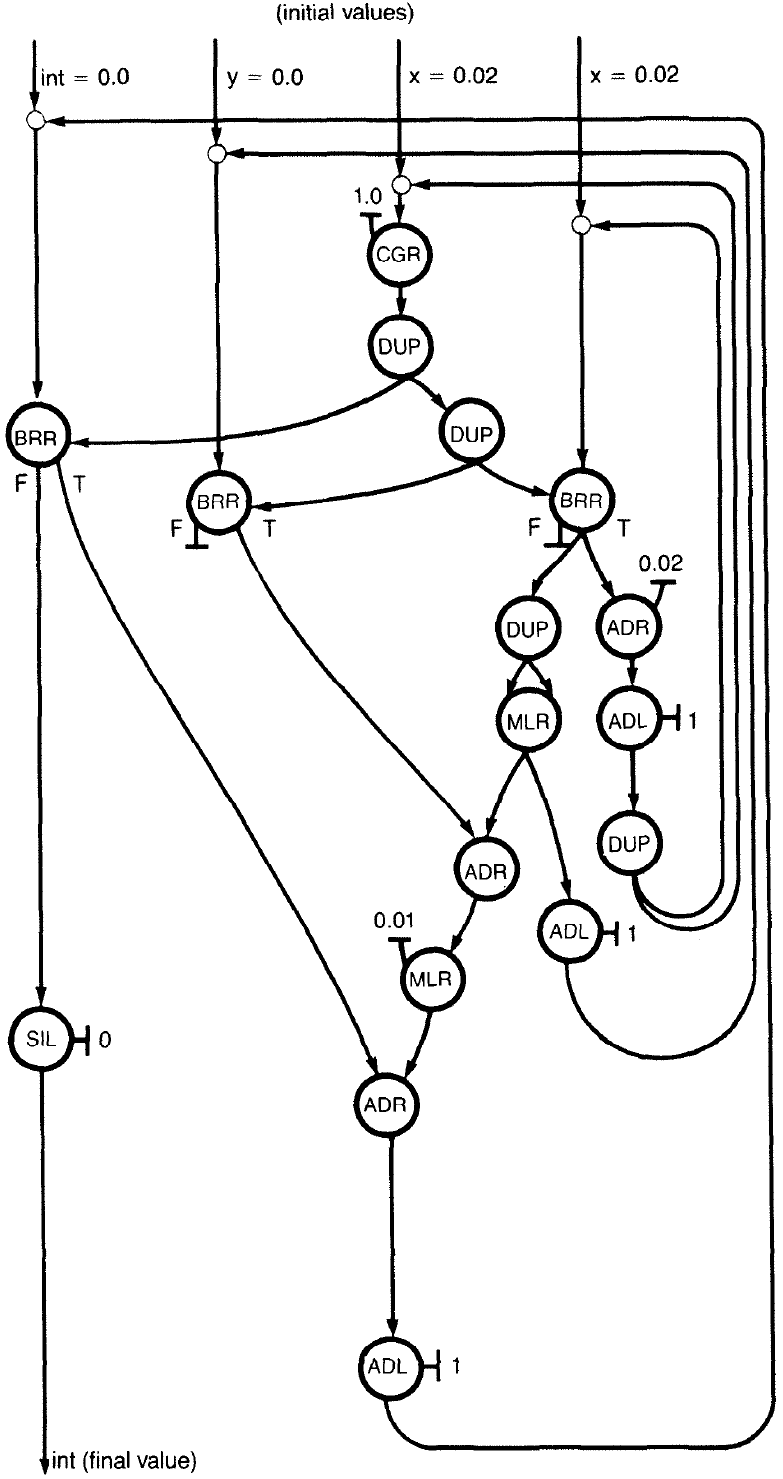
\includegraphics[height=.87\textheight]{programa}
	\end{figure}
\end{frame}

\begin{frame}{Máquina Dataflow de Manchester}
	\subsection{Máquina Dataflow de Manchester}
	\begin{itemize}
		\item Dataflow Dinâmico
		\item Cada pacote é rotulado, identifcando o contexto de cada token, permitindo diferenciá-los em tempo de execução
		\item Permite execução de código reentrante
	\end{itemize}
\end{frame}

\begin{frame}{Token}
	\section{Implementação}
	\subsection{Token}
	
	Tokens de 96 bits
		\begin{itemize}
			\item Dados (37 bits)
			\item Rótulo (36 bits)
			\begin{description}
				\item[Nível de Iteração] Usado para diferenciar tokens de diferentes iterações de um loop
				\item[Nome de Ativação] Diferencia diferentes chamadas de um trecho de código, incluindo chamadas recursivas
				\item[Índice] Usado quando uma mesma operação é aplicada a diversos elementos de uma estrutura de dados
			\end{description}
			\item Destino (22 bits)
			\item Marcador (1 bit)
		\end{itemize}
\end{frame}

\begin{frame}{Token Ring}
	\subsection{Token Ring}
\end{frame}


% Códigos
\begin{frame}{Código Alto Nível}
	\section{Código}
	\subsection{Alto Nível}
	\lstinputlisting[label=lst:sisal,basicstyle=\tiny,frame=single,tabsize=4,caption=Programa exemplo em Sisal]{sisal.txt}
\end{frame}

\begin{frame}{Código Nível Intermediário}
	\subsection{Nível Intermediário}
	\lstinputlisting[label=lst:tass,basicstyle=\tiny,frame=single,tabsize=4,caption=Programa anterior escrito em TASS]{tassPresent.txt}
\end{frame}

\begin{frame}
	\begin{thebibliography}{1}

	\bibitem{IEEEhowto:kopka}
	J. R. GURD, C. C. KIRKHAM, and I. WATSON (1985). {\em THE MANCHESTER PROTOTYPE DATAFLOW COMPUTER}. Communications of the ACM, 28 (1), 34-52.

	\end{thebibliography}
\end{frame}

\end{document}


